\subsubsection{UC12 - Validazione nuovo account registrato}
\begin{figure}[h]
	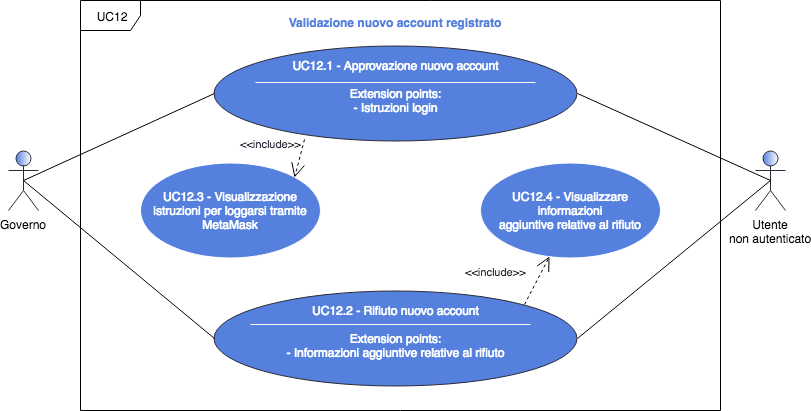
\includegraphics[width=15.5cm]{res/images/UC12Validazione.png} %da adattare in larghezza
	\centering
	\caption{UC12 - Validazione nuovo account registrato}
	
\end{figure}
\begin{itemize}
	\item \textbf{Attori Primari}:
	governo;
	\item \textbf{Attori Secondari}:
	utente non autenticato;
	\item \textbf{Descrizione}: l'account utente può venire rigettato o approvato dal governo;
	\item \textbf{Scenario}: l'utente si è registrato da poco ed attente una risposta da parte del governo in merito alla validazione del proprio account;
	\item \textbf{Precondizione}: l'utente è in coda di attesa per la validazione dell'account;
	\item \textbf{Postcondizione}: l'account utente viene approvato o rigettato. 
\end{itemize}
\subsubsection{UC12.1 - Approvazione nuovo account}
\begin{itemize}
	\item \textbf{Attori Primari}:
	governo;
	\item \textbf{Attori Secondari}:
	utente non autenticato;
	\item \textbf{Descrizione}: l'account utente viene approvato;
	\item \textbf{Scenario}: in seguito alla registrazione, il governo riconosce validi i dati immessi dall'utente;
	\item \textbf{Inclusioni}:
	\begin{itemize}
		\item \textbf{UC12.3}: in seguito all'approvazione dell'account, l'utente visualizza una breve e concisa guida su come loggarsi al sito;
	\end{itemize}
	\item \textbf{Precondizione}: l'utente non ha i permessi per loggarsi al sito;
	\item \textbf{Postcondizione}: l'utente può visualizzare il modo corretto per eseguire il login alla piattaforma.
	
\end{itemize}
\subsubsection{UC12.2 - Rifiuto nuovo account}
\begin{itemize}
	\item \textbf{Attori Primari}:
	governo;
	\item \textbf{Attori Secondari}:
	utente non autenticato;
	\item \textbf{Descrizione}: l'account utente viene rifiutato;
	\item \textbf{Scenario}: in seguito alla registrazione, il governo riconosce non validi i dati immessi dall'utente;
	\item \textbf{Inclusioni}:
	\begin{itemize}
		\item \textbf{UC12.4}: in seguito al rigetto  dell'account, l'utente visualizza dettagli aggiuntivi del perchè non è stato accettato;
	\end{itemize}
	\item \textbf{Precondizione}: l'utente è in attesa di approvazione;
	\item \textbf{Postcondizione}: l'utente può visualizzare ulteriori dettagli in seguito al rifiuto dell'approvazione di validità proprio account.
	
\end{itemize}
\subsubsection{UC12.3 - Visualizzazione istruzioni per loggarsi tramite MetaMask\glosp}
\begin{itemize}
	\item \textbf{Attori Primari}:
	governo;
	\item \textbf{Attori Secondari}:
	utente non autenticato;
	\item \textbf{Descrizione}: l'utente visualizza le istruzioni per procedere al login tramite MetaMask\glosp;
	\item \textbf{Scenario}: in seguito all'approvazione dell'account, l'utente riceve le informazioni necessarie per effettuare tale operazione;
	\item \textbf{Precondizione}:l 'utente non ha idea di come connettersi tramite MetaMask\glosp;
	\item \textbf{Postcondizione}: l'utente ha le abilità necessarie al conseguimento di un login eseguito in modo corretto e sicuro tramite il plugin MetaMask\glosp.
\end{itemize}
\subsubsection{UC12.4 - Visualizzazione informazioni aggiuntive in merito al rigetto dell'account}
\begin{itemize}
	\item \textbf{Attori Primari}:
	governo;
	\item \textbf{Attori Secondari}:
	utente non autenticato;
	\item \textbf{Descrizione}: l'utente visualizza le informazioni aggiuntive relative al rigetto del proprio account;
	\item \textbf{Scenario}: in seguito al rifiuto dell'account, l'utente riceve le informazioni relative a tale rigetto da parte del governo;
	\item \textbf{Precondizione}: l 'utente non ha idea del perchè non è stato accettato;
	\item \textbf{Postcondizione}: l'utente riconosce di aver inserito dati falsi o contenenti errori, pertanto dovrà riprovare la registrazione.
\end{itemize} 
